%%
%% Author: Dario Chinelli
%% begin 2019-12-04
%% last mod 2022-02-02
%%

% Preamble
\documentclass[class=article, crop=false]{standalone}

% Packages
\usepackage{tikz}
\usetikzlibrary{positioning}

% Document
\begin{document}
\fontsmall
\begin{figure}[h]
\centering
\resizebox{0.2\textwidth}{!}{%
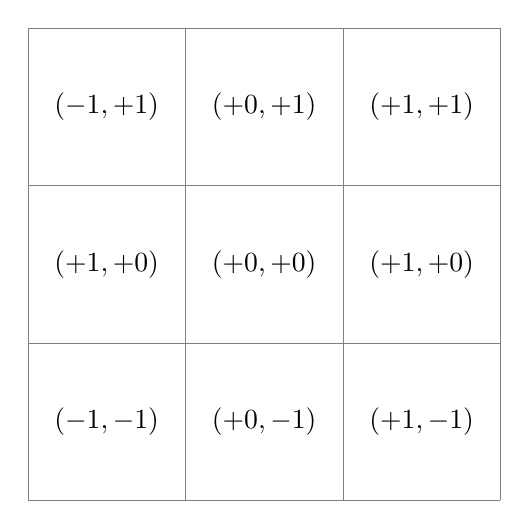
\begin{tikzpicture}
% Lines
\draw[step=2cm, gray, very thin] (0,0) grid (6,6);
% Nodes
\draw (3,3) node[black] {$(+0,+0)$};
\draw (5,3) node[black] {$(+1,+0)$};
\draw (3,5) node[black] {$(+0,+1)$};
\draw (1,3) node[black] {$(+1,+0)$};
\draw (3,1) node[black] {$(+0,-1)$};
\draw (5,5) node[black] {$(+1,+1)$};
\draw (1,5) node[black] {$(-1,+1)$};
\draw (1,1) node[black] {$(-1,-1)$};
\draw (5,1) node[black] {$(+1,-1)$};
\end{tikzpicture}
}%
\captionsetup{width=.5\linewidth}
\caption{Given the initial position at the center square, this is a representation of the change in coordinates to the next cell.}
\label{fig:D2Q9_c}
\end{figure}

\end{document}
